\documentclass{beamer}
\usepackage[english]{babel}
\usepackage[round]{natbib}
\usepackage{color}

% ============================
%  Figures and relative paths
% ============================
\usepackage{graphicx}
\graphicspath{{figures/}}

% =================
%  Beamer options
% =================
\usetheme{default}
\setbeamertemplate{footline}[frame number]
\usecolortheme{rose}

\setbeamerfont{section title}{parent=title}
\setbeamercolor{section title}{parent=titlelike}
%\defbeamertemplate*{section page}{default}[1][]
%{
  %\centering
    %\begin{beamercolorbox}[sep=8pt,center,#1]{section title}
%      \usebeamerfont{section title}\insertsection\par
%    \end{beamercolorbox}
%}
%\newcommand*{\sectionpage}{\usebeamertemplate*{section page}}


% ==========
%  Document
% ==========
\begin{document}

\title{\texttt{rba} Python package}
\date{24/10/2017}
\maketitle

\begin{frame}{Resource Allocation Models}
  \begin{figure}
    \centering
    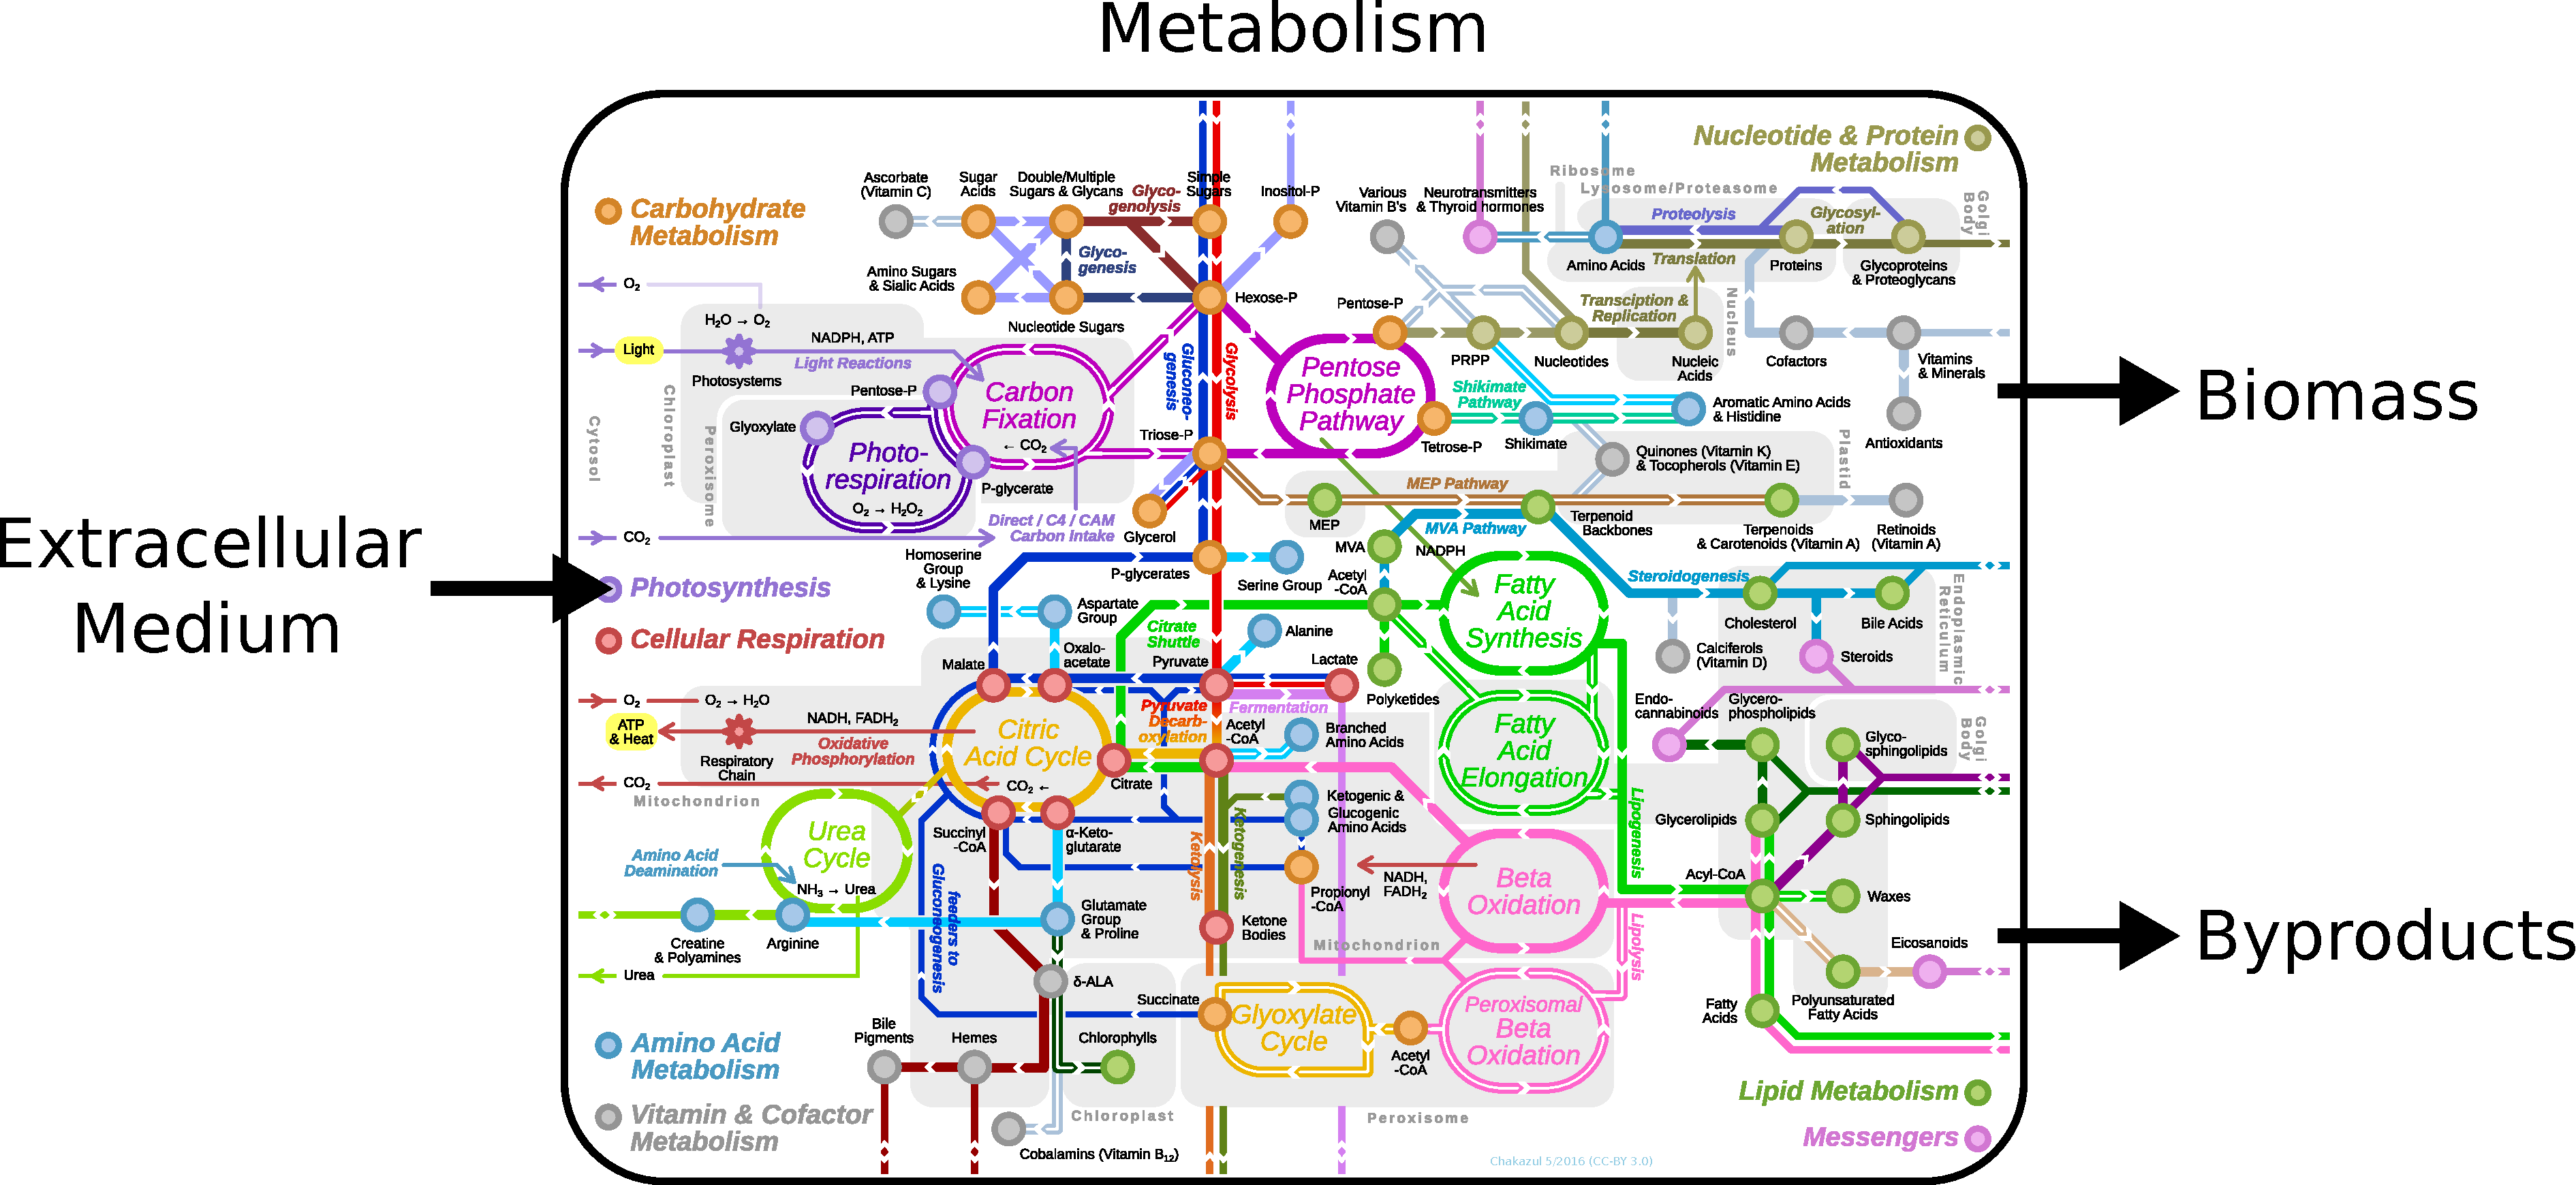
\includegraphics[width=\linewidth]{intro}
  \end{figure}
  3 central constraints:
  \begin{itemize}
    \item Conservation of mass.
    \item Catalytic capacities.
    \item Maximal compartment densities.
  \end{itemize}
\end{frame}

\begin{frame}{RBA constraints}
  Flux Balance Analysis (FBA) models usually provide
  \begin{itemize}
    \item metabolic species
    \item metabolic reactions
    \item biomass targets
  \end{itemize}

  In Resource Balance Analysis (RBA) we also need
  \begin{itemize}
    \item an enzyme-reaction mapping
    \item efficiencies of enzymes
    \item synthesis reactions for enzymes
    and other machineries (ribosome, chaperones)
    \item weight of individual macromolecules
    \item maximal densities for compartments
  \end{itemize}
\end{frame}

\begin{frame}{Automatic generation of synthesis reactions}
  We propose a pipline that extends SBML models with standard information
  to create an RBA model.
  \begin{figure}
    \centering
    
\includegraphics[width=\linewidth]{pipeline_idea}
  \end{figure}
\end{frame}

\begin{frame}{rba Python package}
  The rba package uses three subpackages:
  \begin{figure}
    \centering
    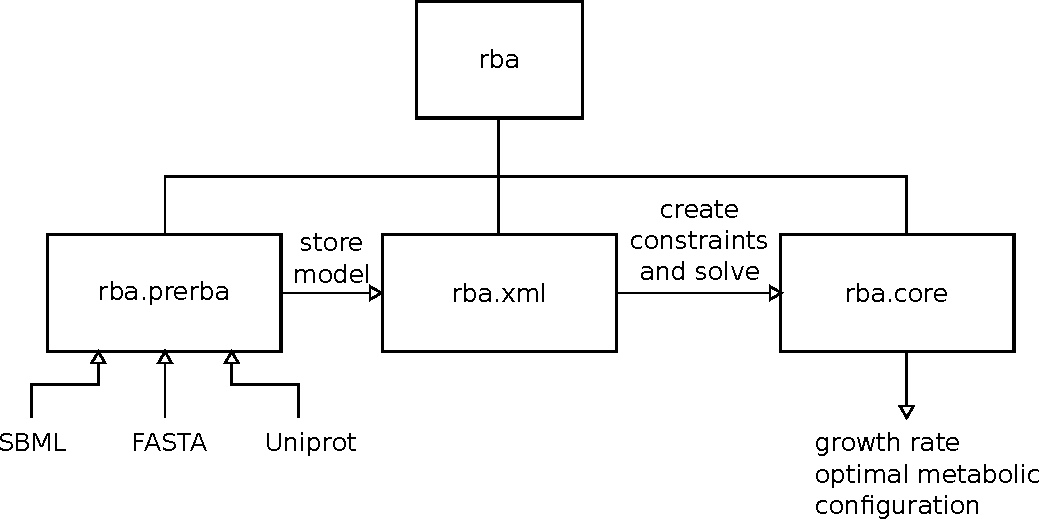
\includegraphics[width=\linewidth]{package_structure}
  \end{figure}
\end{frame}

\begin{frame}{Files needed to run the pipeline.}
  \textbf{Required}
  \begin{itemize}
    \item A general parameter file containing organism ID (template provided).
    \item A valid SBML model (no modification is necessary).
    \item Fasta files (default files with \textit{E. coli} data are provided):
    \begin{itemize}
      \item trnas.fasta: file containing tRNA sequences.
      \item ribosome.fasta: file containing ribosomal RNAs and proteins.
      \item chaperones.fasta: file containing chaperone proteins.
    \end{itemize}
  \end{itemize}
  \textbf{Optional}
  \begin{itemize}
    \item A Uniprot file.
    \item Helper files clarifying ambiguous/missing information.
  \end{itemize}
\end{frame}

\begin{frame}{rba.prerba flow}
  \begin{figure}[!ht]
    \centering
    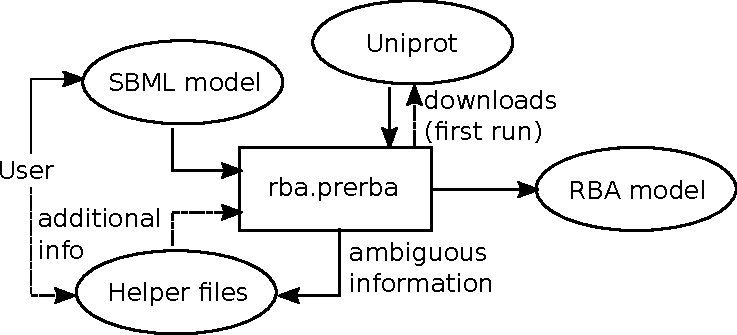
\includegraphics[width=\linewidth]{prerba_summary}
  \end{figure}
  The RBA model uses default values where necessary.
\end{frame}

\begin{frame}{rba.prerba flow}
  \begin{figure}[!ht]
    \centering
    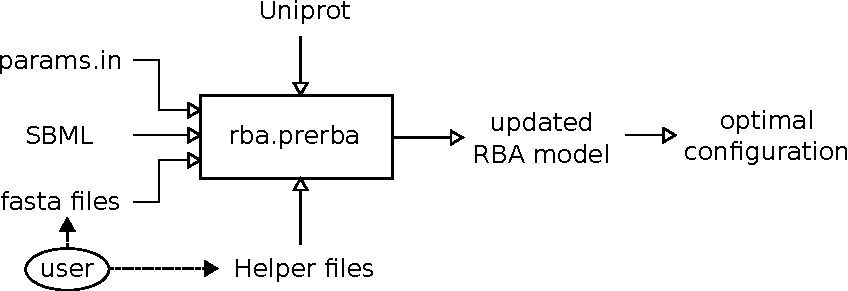
\includegraphics[width=\linewidth]{prerba_summary_2}
  \end{figure}
  The user can provide more accurate values by communicating through
  helper files.
\end{frame}

\begin{frame}{Default values and processes}
  \textbf{Default processes}
  \begin{itemize}
    \item Translation: base for protein synthesis.
    \item Folding: additional synthesis costs for protein synthesis.
    \item Transcription: RNA synthesis.
    \item RNA degradation.
    \item Replication: DNA synthesis.
  \end{itemize}
  \textbf{Default biomass targets}
  \begin{itemize}
    \item maintenance ATP.
    \item production of important metabolites (tRNAs, ATP, etc.).
    \item production of housekeeping proteins.
    \item production of messenger RNAs.
    \item production of DNA.
  \end{itemize}
\end{frame}

\begin{frame}{rba.prerba usage}
  \begin{itemize}
    \item Generate a first model, solve it.
    \item Fill in information in helper files, generate a fully functional
    model.
    \item Adapt enzyme efficiencies using rba.xml.
    \item Add new processes using rba.xml.
  \end{itemize}
\end{frame}

\begin{frame}{Example: \textit{Bacillus subtilis}}
  Expected results with an \emph{hand-curated} RBA model:
  \begin{figure}
    \centering
    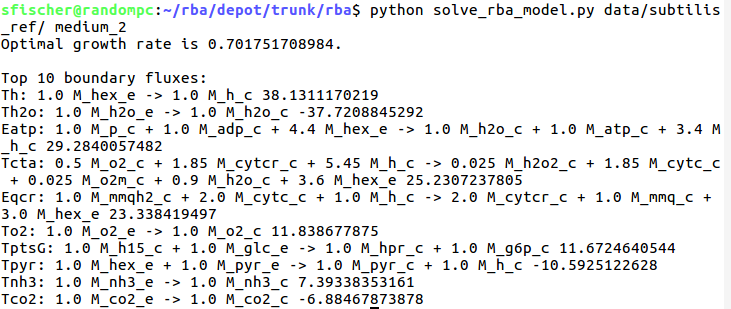
\includegraphics[width=\linewidth]{subtilis_ref}
  \end{figure}
\end{frame}

\begin{frame}{First run from SBML: building model}
  \begin{figure}
    \centering
    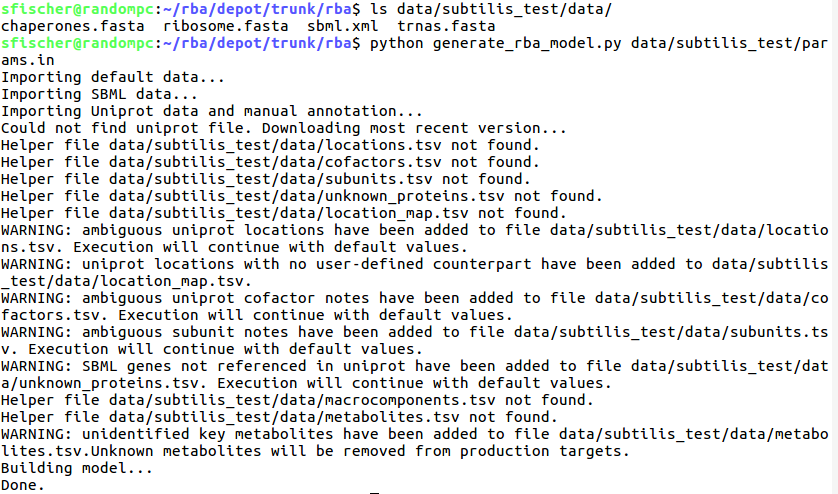
\includegraphics[width=\linewidth]{first_run}
  \end{figure}
\end{frame}

\begin{frame}{First run from SBML: solving}
  \begin{figure}
    \centering
    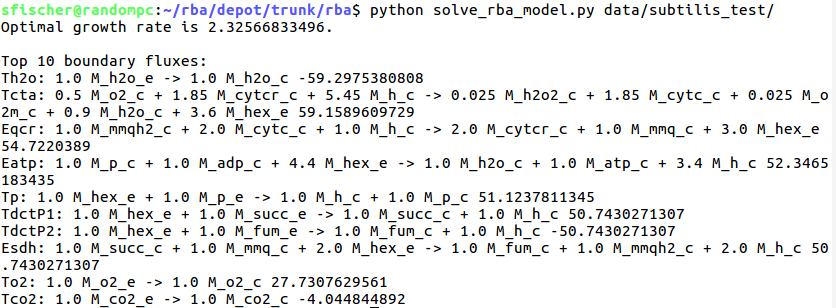
\includegraphics[width=\linewidth]{first_run_solver}
  \end{figure}
\end{frame}

\begin{frame}{Modification of helper files}
  Helper files include information about location, stoichiometry,
  cofactors, etc.
  \begin{figure}
    \centering
    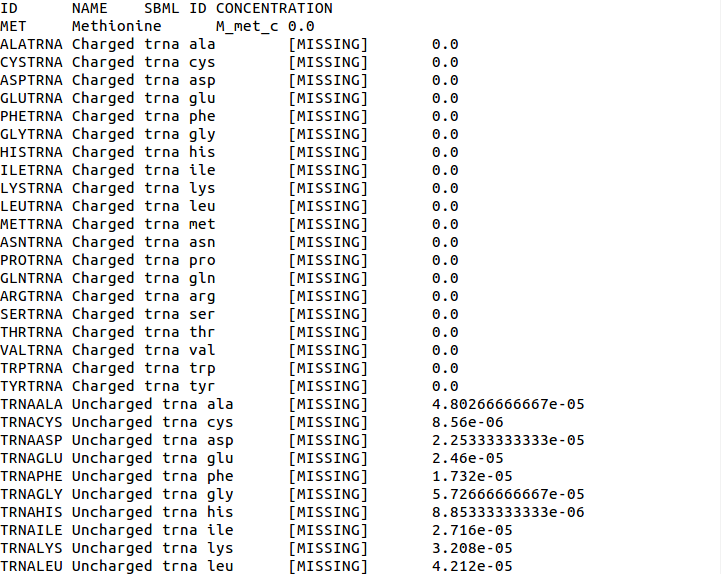
\includegraphics[width=0.8\linewidth]{helper_file_metabolites}
  \end{figure}
\end{frame}

\begin{frame}{Adding metabolite references}
  \begin{figure}
    \centering
    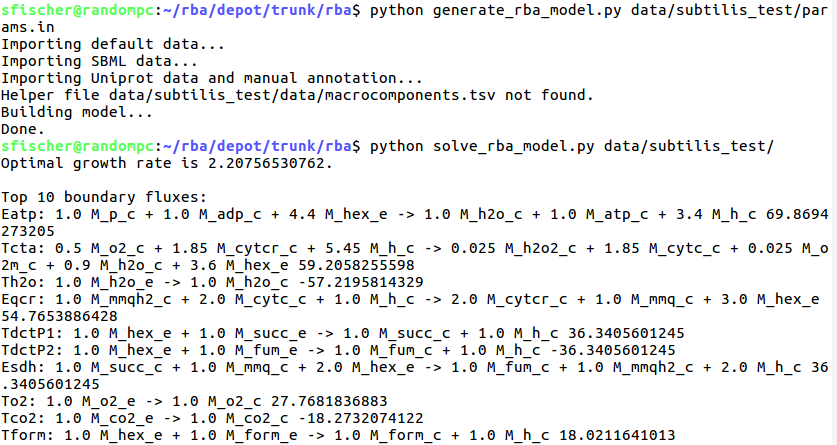
\includegraphics[width=\linewidth]{added_metabolites}
  \end{figure}
\end{frame}

\begin{frame}{Changing medium}
  \begin{figure}
    \centering
    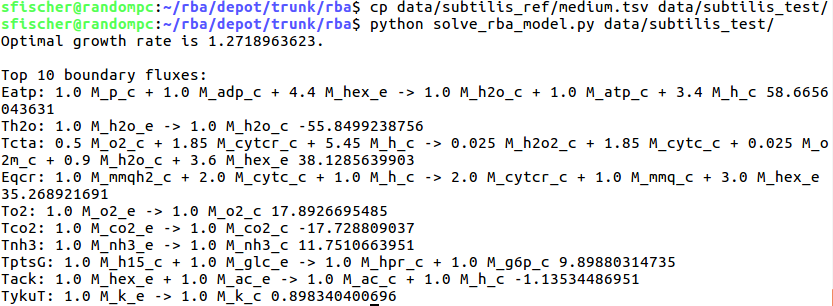
\includegraphics[width=\linewidth]{added_medium}
  \end{figure}
\end{frame}

\begin{frame}{Adding flagella}
  \begin{figure}
    \centering
    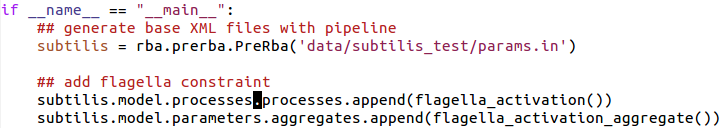
\includegraphics[width=0.9\linewidth]{added_flagella_code_1} \\
    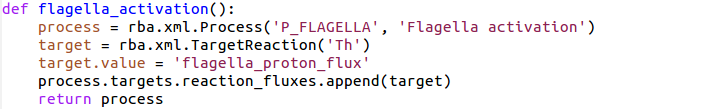
\includegraphics[width=0.9\linewidth]{added_flagella_code_2} \\
    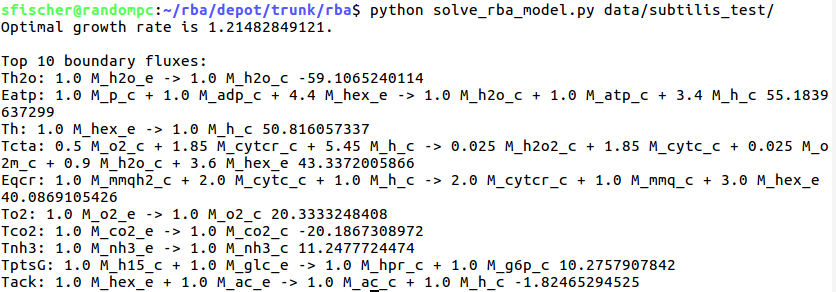
\includegraphics[width=0.9\linewidth]{added_flagella_solver}
  \end{figure}
\end{frame}

\begin{frame}{Adding enzyme efficiencies}
  We dump efficiencies from original model and include simple routine using
  \texttt{rba.xml} to add values to new model.
  \begin{figure}
    \centering
    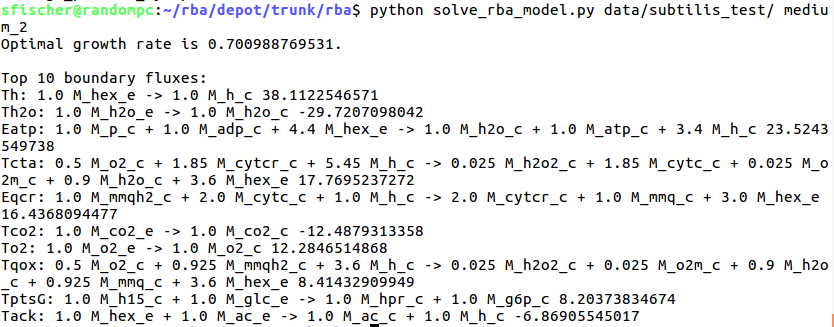
\includegraphics[width=\linewidth]{added_enzyme_efficiencies}
  \end{figure}
\end{frame}


\begin{frame}{Conclusion}
  \begin{itemize}
    \item Efficient assistance to generate an RBA model from an SBML model.
    \item Models are built step-wise, allowing users to see what changed.
    \item XML format that allows user to add routines on top of pipeline.
    \item Efficient solver
    (less than 2s for \textit{B. subtilis}, 15s for \textit{E. coli}).
  \end{itemize}
\end{frame}

\begin{frame}{Perspectives}
  \begin{itemize}
    \item Add data sources, mainly for enzyme efficiencies.
    \item Automatize process building.
    \item Combine our XML format with existing formats.
    \item Add new solver types.
  \end{itemize}
\end{frame}


% ==========
%  Appendix
% ==========
\appendix
\newcounter{finalframe}
\setcounter{finalframe}{\value{framenumber}}

% % % % % % % % % % % ADD APPENDIX FRAMES HERE % % % % % % % % % % % % %

\setcounter{framenumber}{\value{finalframe}}

\end{document}
